% Options for packages loaded elsewhere
\PassOptionsToPackage{unicode}{hyperref}
\PassOptionsToPackage{hyphens}{url}
%
\documentclass[
]{article}
\usepackage{lmodern}
\usepackage{amssymb,amsmath}
\usepackage{ifxetex,ifluatex}
\ifnum 0\ifxetex 1\fi\ifluatex 1\fi=0 % if pdftex
  \usepackage[T1]{fontenc}
  \usepackage[utf8]{inputenc}
  \usepackage{textcomp} % provide euro and other symbols
\else % if luatex or xetex
  \usepackage{unicode-math}
  \defaultfontfeatures{Scale=MatchLowercase}
  \defaultfontfeatures[\rmfamily]{Ligatures=TeX,Scale=1}
\fi
% Use upquote if available, for straight quotes in verbatim environments
\IfFileExists{upquote.sty}{\usepackage{upquote}}{}
\IfFileExists{microtype.sty}{% use microtype if available
  \usepackage[]{microtype}
  \UseMicrotypeSet[protrusion]{basicmath} % disable protrusion for tt fonts
}{}
\makeatletter
\@ifundefined{KOMAClassName}{% if non-KOMA class
  \IfFileExists{parskip.sty}{%
    \usepackage{parskip}
  }{% else
    \setlength{\parindent}{0pt}
    \setlength{\parskip}{6pt plus 2pt minus 1pt}}
}{% if KOMA class
  \KOMAoptions{parskip=half}}
\makeatother
\usepackage{xcolor}
\IfFileExists{xurl.sty}{\usepackage{xurl}}{} % add URL line breaks if available
\IfFileExists{bookmark.sty}{\usepackage{bookmark}}{\usepackage{hyperref}}
\hypersetup{
  pdftitle={HW3},
  pdfauthor={Nikhil Gopal},
  hidelinks,
  pdfcreator={LaTeX via pandoc}}
\urlstyle{same} % disable monospaced font for URLs
\usepackage[margin=1in]{geometry}
\usepackage{color}
\usepackage{fancyvrb}
\newcommand{\VerbBar}{|}
\newcommand{\VERB}{\Verb[commandchars=\\\{\}]}
\DefineVerbatimEnvironment{Highlighting}{Verbatim}{commandchars=\\\{\}}
% Add ',fontsize=\small' for more characters per line
\usepackage{framed}
\definecolor{shadecolor}{RGB}{248,248,248}
\newenvironment{Shaded}{\begin{snugshade}}{\end{snugshade}}
\newcommand{\AlertTok}[1]{\textcolor[rgb]{0.94,0.16,0.16}{#1}}
\newcommand{\AnnotationTok}[1]{\textcolor[rgb]{0.56,0.35,0.01}{\textbf{\textit{#1}}}}
\newcommand{\AttributeTok}[1]{\textcolor[rgb]{0.77,0.63,0.00}{#1}}
\newcommand{\BaseNTok}[1]{\textcolor[rgb]{0.00,0.00,0.81}{#1}}
\newcommand{\BuiltInTok}[1]{#1}
\newcommand{\CharTok}[1]{\textcolor[rgb]{0.31,0.60,0.02}{#1}}
\newcommand{\CommentTok}[1]{\textcolor[rgb]{0.56,0.35,0.01}{\textit{#1}}}
\newcommand{\CommentVarTok}[1]{\textcolor[rgb]{0.56,0.35,0.01}{\textbf{\textit{#1}}}}
\newcommand{\ConstantTok}[1]{\textcolor[rgb]{0.00,0.00,0.00}{#1}}
\newcommand{\ControlFlowTok}[1]{\textcolor[rgb]{0.13,0.29,0.53}{\textbf{#1}}}
\newcommand{\DataTypeTok}[1]{\textcolor[rgb]{0.13,0.29,0.53}{#1}}
\newcommand{\DecValTok}[1]{\textcolor[rgb]{0.00,0.00,0.81}{#1}}
\newcommand{\DocumentationTok}[1]{\textcolor[rgb]{0.56,0.35,0.01}{\textbf{\textit{#1}}}}
\newcommand{\ErrorTok}[1]{\textcolor[rgb]{0.64,0.00,0.00}{\textbf{#1}}}
\newcommand{\ExtensionTok}[1]{#1}
\newcommand{\FloatTok}[1]{\textcolor[rgb]{0.00,0.00,0.81}{#1}}
\newcommand{\FunctionTok}[1]{\textcolor[rgb]{0.00,0.00,0.00}{#1}}
\newcommand{\ImportTok}[1]{#1}
\newcommand{\InformationTok}[1]{\textcolor[rgb]{0.56,0.35,0.01}{\textbf{\textit{#1}}}}
\newcommand{\KeywordTok}[1]{\textcolor[rgb]{0.13,0.29,0.53}{\textbf{#1}}}
\newcommand{\NormalTok}[1]{#1}
\newcommand{\OperatorTok}[1]{\textcolor[rgb]{0.81,0.36,0.00}{\textbf{#1}}}
\newcommand{\OtherTok}[1]{\textcolor[rgb]{0.56,0.35,0.01}{#1}}
\newcommand{\PreprocessorTok}[1]{\textcolor[rgb]{0.56,0.35,0.01}{\textit{#1}}}
\newcommand{\RegionMarkerTok}[1]{#1}
\newcommand{\SpecialCharTok}[1]{\textcolor[rgb]{0.00,0.00,0.00}{#1}}
\newcommand{\SpecialStringTok}[1]{\textcolor[rgb]{0.31,0.60,0.02}{#1}}
\newcommand{\StringTok}[1]{\textcolor[rgb]{0.31,0.60,0.02}{#1}}
\newcommand{\VariableTok}[1]{\textcolor[rgb]{0.00,0.00,0.00}{#1}}
\newcommand{\VerbatimStringTok}[1]{\textcolor[rgb]{0.31,0.60,0.02}{#1}}
\newcommand{\WarningTok}[1]{\textcolor[rgb]{0.56,0.35,0.01}{\textbf{\textit{#1}}}}
\usepackage{graphicx,grffile}
\makeatletter
\def\maxwidth{\ifdim\Gin@nat@width>\linewidth\linewidth\else\Gin@nat@width\fi}
\def\maxheight{\ifdim\Gin@nat@height>\textheight\textheight\else\Gin@nat@height\fi}
\makeatother
% Scale images if necessary, so that they will not overflow the page
% margins by default, and it is still possible to overwrite the defaults
% using explicit options in \includegraphics[width, height, ...]{}
\setkeys{Gin}{width=\maxwidth,height=\maxheight,keepaspectratio}
% Set default figure placement to htbp
\makeatletter
\def\fps@figure{htbp}
\makeatother
\setlength{\emergencystretch}{3em} % prevent overfull lines
\providecommand{\tightlist}{%
  \setlength{\itemsep}{0pt}\setlength{\parskip}{0pt}}
\setcounter{secnumdepth}{-\maxdimen} % remove section numbering

\title{HW3}
\author{Nikhil Gopal}
\date{10/25/2021}

\begin{document}
\maketitle

\begin{Shaded}
\begin{Highlighting}[]
\KeywordTok{rm}\NormalTok{(}\DataTypeTok{list =} \KeywordTok{ls}\NormalTok{())}
\KeywordTok{library}\NormalTok{(raster)}
\end{Highlighting}
\end{Shaded}

\begin{verbatim}
## Loading required package: sp
\end{verbatim}

\begin{verbatim}
## Warning: package 'sp' was built under R version 4.0.3
\end{verbatim}

\begin{Shaded}
\begin{Highlighting}[]
\KeywordTok{library}\NormalTok{(glmnet)}
\end{Highlighting}
\end{Shaded}

\begin{verbatim}
## Warning: package 'glmnet' was built under R version 4.0.3
\end{verbatim}

\begin{verbatim}
## Loading required package: Matrix
\end{verbatim}

\begin{verbatim}
## Loaded glmnet 4.1
\end{verbatim}

\begin{Shaded}
\begin{Highlighting}[]
\KeywordTok{library}\NormalTok{(dplyr)}
\end{Highlighting}
\end{Shaded}

\begin{verbatim}
## 
## Attaching package: 'dplyr'
\end{verbatim}

\begin{verbatim}
## The following objects are masked from 'package:raster':
## 
##     intersect, select, union
\end{verbatim}

\begin{verbatim}
## The following objects are masked from 'package:stats':
## 
##     filter, lag
\end{verbatim}

\begin{verbatim}
## The following objects are masked from 'package:base':
## 
##     intersect, setdiff, setequal, union
\end{verbatim}

\begin{Shaded}
\begin{Highlighting}[]
\KeywordTok{setwd}\NormalTok{(}\StringTok{"G:/My Drive/STAT 3105/HW3/"}\NormalTok{)}
\end{Highlighting}
\end{Shaded}

\textbf{1a Does one/none/both of the cost functions encourage sparse
estimates? If so, which one? Explain your answer.}

The q = 0.5 cost function encourages sparce estimates. Relative to the
other function, this function provides \(l_i\) that are closer to the
origin on average. From looking at the constraint regions for the
parameters, we know that the 0.5 function would encourage sparce
estimates.

\textbf{1b Which of the points x1, . . . , x5 would achieve the smallest
cost under the `q-constrained least squares cost function? For each of
the two cases, name the respective point and give a brief explanation
for your answer. }

For q = 0.5, beta becomes zero when the line intersects the beta1 axis,
which occurs at point x3.

For q = 4, beta becomes zero when the line intersects the ellipse, which
occurs at point x4.

\textbf{1c Write down the loss function with q = 0.5 and q = 4
respectively. Which one do you think is easier to solve numerically and
why?}

Loss q = 4:

\[\mathcal{L}_{\lambda, 4} = \sum_{i = 1}^n (y_i - \sum_{j = 1}^2 x_j\beta_j)^2 + \lambda (\sum_{i = 1}^2 |\beta_i|^{4})^{\frac{1}{4}}\]
Loss q = 0.5:

\[\mathcal{L}_{\lambda, 0.5} = \sum_{i = 1}^n (y_i - \sum_{j = 1}^2 x_j\beta_j)^2 + \lambda (\sum_{i = 1}^2 |\beta_i|^{0.5})^{\frac{1}{0.5}}\]

The convex function (q = 4) would be easier to solve. As shown on the
diagrams in the lecture, local minimums are global minimums for convex
functions, whereas with nonconvex functions, one cannot be sure that a
local minimum is a global minimum. Thus, finding one local minimum is
sufficient to solve a convex loss function, making it easier to solve
overall.

\textbf{2a Using the 5 penalty values of λ mentioned above to fit the
ridge regression model. You will have the coefficient β ∈ R16384.
Reshape β into 128 × 128 matrix, and plot the matrix as in the original
image. Which coefficient yields the best result?}

\begin{Shaded}
\begin{Highlighting}[]
\NormalTok{X_mat <-}\StringTok{ }\KeywordTok{as.matrix}\NormalTok{(}\KeywordTok{read.table}\NormalTok{(}\DataTypeTok{file =} \StringTok{"hw3_Q2_X.txt"}\NormalTok{))}

\NormalTok{Y_lst <-}\StringTok{ }\KeywordTok{as.matrix}\NormalTok{(}\KeywordTok{read.table}\NormalTok{(}\StringTok{"hw3_Q2_Y.txt"}\NormalTok{))}

\CommentTok{# Ridge Regression (alpha = 0)}
\NormalTok{ridge_reg1 <-}\StringTok{ }\KeywordTok{glmnet}\NormalTok{(X_mat, Y_lst, }\DataTypeTok{family =} \StringTok{"gaussian"}\NormalTok{, }\DataTypeTok{intercept =}\NormalTok{ T,}
\DataTypeTok{alpha=}\DecValTok{0}\NormalTok{, }\DataTypeTok{lambda =} \FloatTok{0.000001}\NormalTok{, }\DataTypeTok{lambda.min.ratio =} \FloatTok{1e-8}\NormalTok{,}
\DataTypeTok{standardize =}\NormalTok{ F, }\DataTypeTok{nlambda =} \DecValTok{1}\NormalTok{)}

\NormalTok{ridge_reg2 <-}\StringTok{ }\KeywordTok{glmnet}\NormalTok{(X_mat, Y_lst, }\DataTypeTok{family =} \StringTok{"gaussian"}\NormalTok{, }\DataTypeTok{intercept =}\NormalTok{ T,}
\DataTypeTok{alpha=}\DecValTok{0}\NormalTok{, }\DataTypeTok{lambda =} \FloatTok{0.0001}\NormalTok{, }\DataTypeTok{lambda.min.ratio =} \FloatTok{1e-8}\NormalTok{,}
\DataTypeTok{standardize =}\NormalTok{ F, }\DataTypeTok{nlambda =} \DecValTok{1}\NormalTok{)}

\NormalTok{ridge_reg3 <-}\StringTok{ }\KeywordTok{glmnet}\NormalTok{(X_mat, Y_lst, }\DataTypeTok{family =} \StringTok{"gaussian"}\NormalTok{, }\DataTypeTok{intercept =}\NormalTok{ T,}
\DataTypeTok{alpha=}\DecValTok{0}\NormalTok{, }\DataTypeTok{lambda =} \FloatTok{0.01}\NormalTok{, }\DataTypeTok{lambda.min.ratio =} \FloatTok{1e-8}\NormalTok{,}
\DataTypeTok{standardize =}\NormalTok{ F, }\DataTypeTok{nlambda =} \DecValTok{1}\NormalTok{)}

\NormalTok{ridge_reg4 <-}\StringTok{ }\KeywordTok{glmnet}\NormalTok{(X_mat, Y_lst, }\DataTypeTok{family =} \StringTok{"gaussian"}\NormalTok{, }\DataTypeTok{intercept =}\NormalTok{ T,}
\DataTypeTok{alpha=}\DecValTok{0}\NormalTok{, }\DataTypeTok{lambda =} \FloatTok{0.1}\NormalTok{, }\DataTypeTok{lambda.min.ratio =} \FloatTok{1e-8}\NormalTok{,}
\DataTypeTok{standardize =}\NormalTok{ F, }\DataTypeTok{nlambda =} \DecValTok{1}\NormalTok{)}

\NormalTok{ridge_reg5 <-}\StringTok{ }\KeywordTok{glmnet}\NormalTok{(X_mat, Y_lst, }\DataTypeTok{family =} \StringTok{"gaussian"}\NormalTok{, }\DataTypeTok{intercept =}\NormalTok{ T,}
\DataTypeTok{alpha=}\DecValTok{0}\NormalTok{, }\DataTypeTok{lambda =} \DecValTok{1}\NormalTok{, }\DataTypeTok{lambda.min.ratio =} \FloatTok{1e-8}\NormalTok{,}
\DataTypeTok{standardize =}\NormalTok{ F, }\DataTypeTok{nlambda =} \DecValTok{1}\NormalTok{)}

\CommentTok{# Reshape Ridge Coefficients to a 128x128 matrix}
\NormalTok{beta_mat6 <-}\StringTok{ }\KeywordTok{matrix}\NormalTok{(ridge_reg1}\OperatorTok{$}\NormalTok{beta[,}\DecValTok{1}\NormalTok{], }\DataTypeTok{nrow=}\DecValTok{128}\NormalTok{, }\DataTypeTok{byrow=}\NormalTok{T)}
\NormalTok{beta_mat7 <-}\StringTok{ }\KeywordTok{matrix}\NormalTok{(ridge_reg2}\OperatorTok{$}\NormalTok{beta[,}\DecValTok{1}\NormalTok{], }\DataTypeTok{nrow=}\DecValTok{128}\NormalTok{, }\DataTypeTok{byrow=}\NormalTok{T)}
\NormalTok{beta_mat8 <-}\StringTok{ }\KeywordTok{matrix}\NormalTok{(ridge_reg3}\OperatorTok{$}\NormalTok{beta[,}\DecValTok{1}\NormalTok{], }\DataTypeTok{nrow=}\DecValTok{128}\NormalTok{, }\DataTypeTok{byrow=}\NormalTok{T)}
\NormalTok{beta_mat9 <-}\StringTok{ }\KeywordTok{matrix}\NormalTok{(ridge_reg4}\OperatorTok{$}\NormalTok{beta[,}\DecValTok{1}\NormalTok{], }\DataTypeTok{nrow=}\DecValTok{128}\NormalTok{, }\DataTypeTok{byrow=}\NormalTok{T)}
\NormalTok{beta_mat10 <-}\StringTok{ }\KeywordTok{matrix}\NormalTok{(ridge_reg5}\OperatorTok{$}\NormalTok{beta[,}\DecValTok{1}\NormalTok{], }\DataTypeTok{nrow=}\DecValTok{128}\NormalTok{, }\DataTypeTok{byrow=}\NormalTok{T)}

\CommentTok{# Visualize the Matrix in Grey Scale}
\KeywordTok{image}\NormalTok{(}\KeywordTok{t}\NormalTok{(}\KeywordTok{apply}\NormalTok{(beta_mat6, }\DecValTok{2}\NormalTok{, rev)), }\DataTypeTok{col=}\KeywordTok{grey}\NormalTok{(}\KeywordTok{seq}\NormalTok{(}\DecValTok{0}\NormalTok{, }\DecValTok{1}\NormalTok{, }\DataTypeTok{length=}\DecValTok{256}\NormalTok{)), }\DataTypeTok{main =} \StringTok{"Lambda = 0.000001"}\NormalTok{)}
\end{Highlighting}
\end{Shaded}

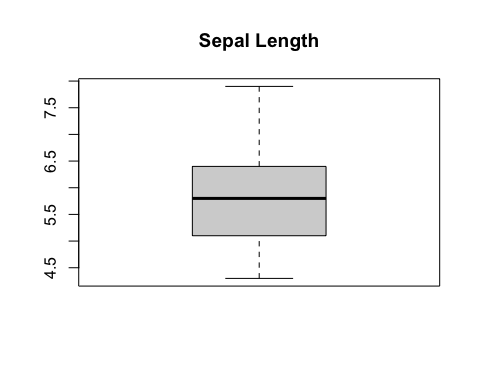
\includegraphics{HW3_files/figure-latex/unnamed-chunk-2-1.pdf}

\begin{Shaded}
\begin{Highlighting}[]
\KeywordTok{image}\NormalTok{(}\KeywordTok{t}\NormalTok{(}\KeywordTok{apply}\NormalTok{(beta_mat7, }\DecValTok{2}\NormalTok{, rev)), }\DataTypeTok{col=}\KeywordTok{grey}\NormalTok{(}\KeywordTok{seq}\NormalTok{(}\DecValTok{0}\NormalTok{, }\DecValTok{1}\NormalTok{, }\DataTypeTok{length=}\DecValTok{256}\NormalTok{)), }\DataTypeTok{main =} \StringTok{"Lambda = 0.0001"}\NormalTok{)}
\end{Highlighting}
\end{Shaded}

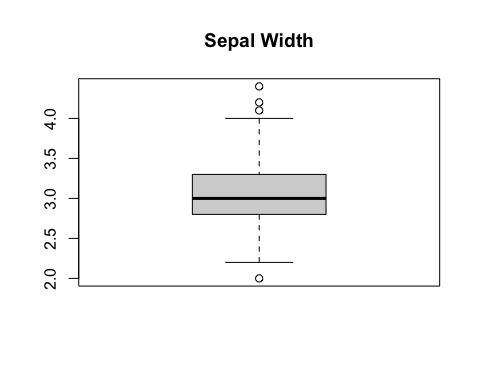
\includegraphics{HW3_files/figure-latex/unnamed-chunk-2-2.pdf}

\begin{Shaded}
\begin{Highlighting}[]
\KeywordTok{image}\NormalTok{(}\KeywordTok{t}\NormalTok{(}\KeywordTok{apply}\NormalTok{(beta_mat8, }\DecValTok{2}\NormalTok{, rev)), }\DataTypeTok{col=}\KeywordTok{grey}\NormalTok{(}\KeywordTok{seq}\NormalTok{(}\DecValTok{0}\NormalTok{, }\DecValTok{1}\NormalTok{, }\DataTypeTok{length=}\DecValTok{256}\NormalTok{)), }\DataTypeTok{main =} \StringTok{"0.01"}\NormalTok{)}
\end{Highlighting}
\end{Shaded}

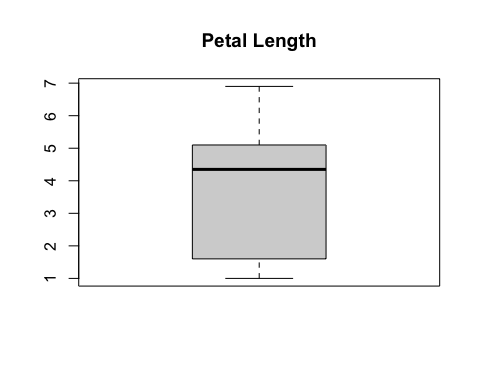
\includegraphics{HW3_files/figure-latex/unnamed-chunk-2-3.pdf}

\begin{Shaded}
\begin{Highlighting}[]
\KeywordTok{image}\NormalTok{(}\KeywordTok{t}\NormalTok{(}\KeywordTok{apply}\NormalTok{(beta_mat9, }\DecValTok{2}\NormalTok{, rev)), }\DataTypeTok{col=}\KeywordTok{grey}\NormalTok{(}\KeywordTok{seq}\NormalTok{(}\DecValTok{0}\NormalTok{, }\DecValTok{1}\NormalTok{, }\DataTypeTok{length=}\DecValTok{256}\NormalTok{)), }\DataTypeTok{main =} \StringTok{"0.1"}\NormalTok{)}
\end{Highlighting}
\end{Shaded}

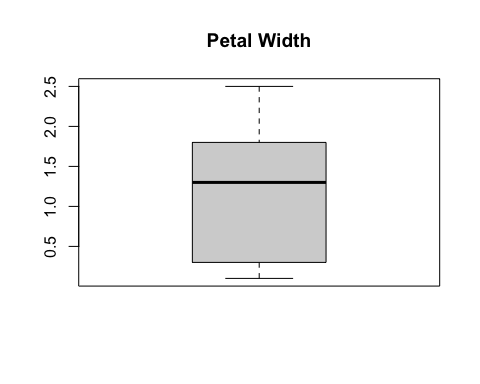
\includegraphics{HW3_files/figure-latex/unnamed-chunk-2-4.pdf}

\begin{Shaded}
\begin{Highlighting}[]
\KeywordTok{image}\NormalTok{(}\KeywordTok{t}\NormalTok{(}\KeywordTok{apply}\NormalTok{(beta_mat10, }\DecValTok{2}\NormalTok{, rev)), }\DataTypeTok{col=}\KeywordTok{grey}\NormalTok{(}\KeywordTok{seq}\NormalTok{(}\DecValTok{0}\NormalTok{, }\DecValTok{1}\NormalTok{, }\DataTypeTok{length=}\DecValTok{256}\NormalTok{)), }\DataTypeTok{main =} \StringTok{"1"}\NormalTok{)}
\end{Highlighting}
\end{Shaded}

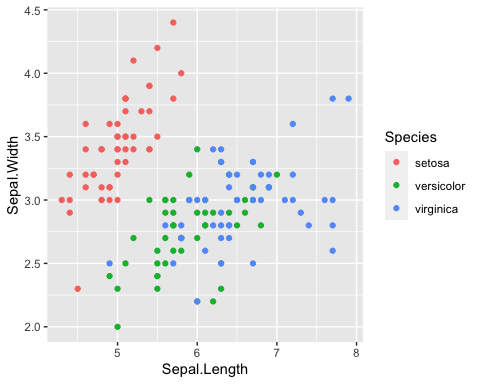
\includegraphics{HW3_files/figure-latex/unnamed-chunk-2-5.pdf}

The ridge model with lambda = 0.1 yielded the best results.

\textbf{2b Using the 5 penalty values of λ mentioned above to fit the
lasso model. You will have the coefficient β ∈ R 16384. Reshape β into
128 × 128 matrix, and plot the matrix as in the original image. Which
coefficient yields the best result? }

\begin{Shaded}
\begin{Highlighting}[]
\CommentTok{#import data}




\CommentTok{# Lasso Regression (alpha = 1)}
\NormalTok{lasso_reg1 <-}\StringTok{ }\KeywordTok{glmnet}\NormalTok{(X_mat, Y_lst, }\DataTypeTok{family =} \StringTok{"gaussian"}\NormalTok{, }\DataTypeTok{intercept =}\NormalTok{ T,}
\DataTypeTok{alpha=}\DecValTok{1}\NormalTok{, }\DataTypeTok{lambda =} \FloatTok{0.000001}\NormalTok{, }\DataTypeTok{lambda.min.ratio =} \FloatTok{1e-8}\NormalTok{,}
\DataTypeTok{standardize =}\NormalTok{ F, }\DataTypeTok{nlambda =} \DecValTok{1}\NormalTok{)}

\NormalTok{lasso_reg2 <-}\StringTok{ }\KeywordTok{glmnet}\NormalTok{(X_mat, Y_lst, }\DataTypeTok{family =} \StringTok{"gaussian"}\NormalTok{, }\DataTypeTok{intercept =}\NormalTok{ T,}
\DataTypeTok{alpha=}\DecValTok{1}\NormalTok{, }\DataTypeTok{lambda =} \FloatTok{0.0001}\NormalTok{, }\DataTypeTok{lambda.min.ratio =} \FloatTok{1e-8}\NormalTok{,}
\DataTypeTok{standardize =}\NormalTok{ F, }\DataTypeTok{nlambda =} \DecValTok{1}\NormalTok{)}

\NormalTok{lasso_reg3 <-}\StringTok{ }\KeywordTok{glmnet}\NormalTok{(X_mat, Y_lst, }\DataTypeTok{family =} \StringTok{"gaussian"}\NormalTok{, }\DataTypeTok{intercept =}\NormalTok{ T,}
\DataTypeTok{alpha=}\DecValTok{1}\NormalTok{, }\DataTypeTok{lambda =} \FloatTok{0.01}\NormalTok{, }\DataTypeTok{lambda.min.ratio =} \FloatTok{1e-8}\NormalTok{,}
\DataTypeTok{standardize =}\NormalTok{ F, }\DataTypeTok{nlambda =} \DecValTok{1}\NormalTok{)}

\NormalTok{lasso_reg4 <-}\StringTok{ }\KeywordTok{glmnet}\NormalTok{(X_mat, Y_lst, }\DataTypeTok{family =} \StringTok{"gaussian"}\NormalTok{, }\DataTypeTok{intercept =}\NormalTok{ T,}
\DataTypeTok{alpha=}\DecValTok{1}\NormalTok{, }\DataTypeTok{lambda =} \FloatTok{0.1}\NormalTok{, }\DataTypeTok{lambda.min.ratio =} \FloatTok{1e-8}\NormalTok{,}
\DataTypeTok{standardize =}\NormalTok{ F, }\DataTypeTok{nlambda =} \DecValTok{1}\NormalTok{)}

\NormalTok{lasso_reg5 <-}\StringTok{ }\KeywordTok{glmnet}\NormalTok{(X_mat, Y_lst, }\DataTypeTok{family =} \StringTok{"gaussian"}\NormalTok{, }\DataTypeTok{intercept =}\NormalTok{ T,}
\DataTypeTok{alpha=}\DecValTok{1}\NormalTok{, }\DataTypeTok{lambda =} \DecValTok{1}\NormalTok{, }\DataTypeTok{lambda.min.ratio =} \FloatTok{1e-8}\NormalTok{,}
\DataTypeTok{standardize =}\NormalTok{ F, }\DataTypeTok{nlambda =} \DecValTok{1}\NormalTok{)}


\CommentTok{# Reshape Lasso Coefficients to a 128x128 matrix}
\NormalTok{beta_mat1 <-}\StringTok{ }\KeywordTok{matrix}\NormalTok{(lasso_reg1}\OperatorTok{$}\NormalTok{beta[,}\DecValTok{1}\NormalTok{], }\DataTypeTok{nrow=}\DecValTok{128}\NormalTok{, }\DataTypeTok{byrow=}\NormalTok{T)}
\NormalTok{beta_mat2 <-}\StringTok{ }\KeywordTok{matrix}\NormalTok{(lasso_reg2}\OperatorTok{$}\NormalTok{beta[,}\DecValTok{1}\NormalTok{], }\DataTypeTok{nrow=}\DecValTok{128}\NormalTok{, }\DataTypeTok{byrow=}\NormalTok{T)}
\NormalTok{beta_mat3 <-}\StringTok{ }\KeywordTok{matrix}\NormalTok{(lasso_reg3}\OperatorTok{$}\NormalTok{beta[,}\DecValTok{1}\NormalTok{], }\DataTypeTok{nrow=}\DecValTok{128}\NormalTok{, }\DataTypeTok{byrow=}\NormalTok{T)}
\NormalTok{beta_mat4 <-}\StringTok{ }\KeywordTok{matrix}\NormalTok{(lasso_reg4}\OperatorTok{$}\NormalTok{beta[,}\DecValTok{1}\NormalTok{], }\DataTypeTok{nrow=}\DecValTok{128}\NormalTok{, }\DataTypeTok{byrow=}\NormalTok{T)}
\NormalTok{beta_mat5 <-}\StringTok{ }\KeywordTok{matrix}\NormalTok{(lasso_reg5}\OperatorTok{$}\NormalTok{beta[,}\DecValTok{1}\NormalTok{], }\DataTypeTok{nrow=}\DecValTok{128}\NormalTok{, }\DataTypeTok{byrow=}\NormalTok{T)}


\CommentTok{# Visualize the Matrix in Grey Scale}
\KeywordTok{image}\NormalTok{(}\KeywordTok{t}\NormalTok{(}\KeywordTok{apply}\NormalTok{(beta_mat1, }\DecValTok{2}\NormalTok{, rev)), }\DataTypeTok{col=}\KeywordTok{grey}\NormalTok{(}\KeywordTok{seq}\NormalTok{(}\DecValTok{0}\NormalTok{, }\DecValTok{1}\NormalTok{, }\DataTypeTok{length=}\DecValTok{256}\NormalTok{)), }\DataTypeTok{main =} \StringTok{"Lambda = 0.000001"}\NormalTok{)}
\end{Highlighting}
\end{Shaded}

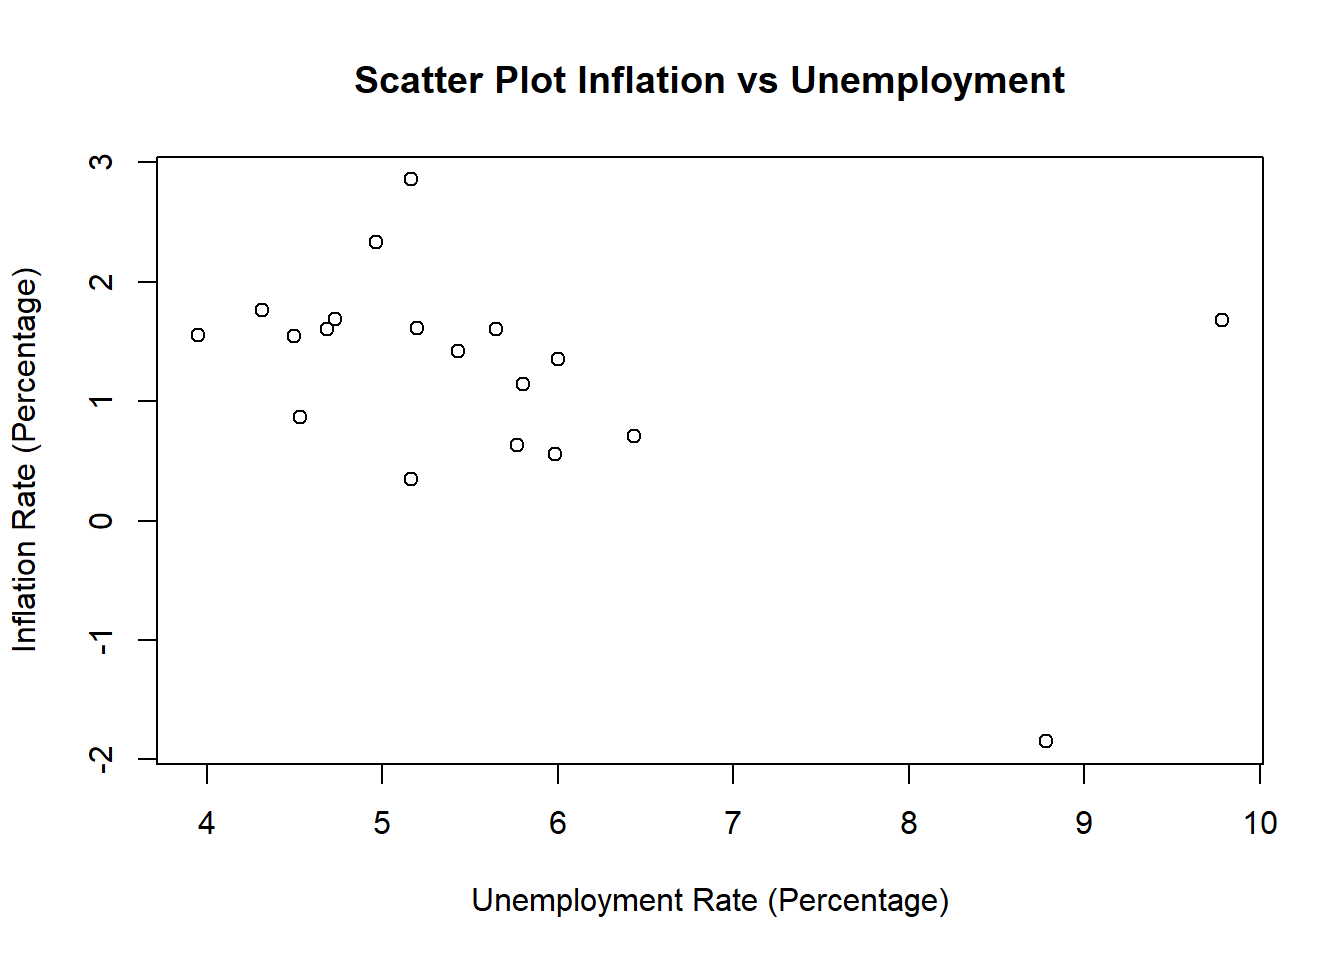
\includegraphics{HW3_files/figure-latex/unnamed-chunk-3-1.pdf}

\begin{Shaded}
\begin{Highlighting}[]
\KeywordTok{image}\NormalTok{(}\KeywordTok{t}\NormalTok{(}\KeywordTok{apply}\NormalTok{(beta_mat2, }\DecValTok{2}\NormalTok{, rev)), }\DataTypeTok{col=}\KeywordTok{grey}\NormalTok{(}\KeywordTok{seq}\NormalTok{(}\DecValTok{0}\NormalTok{, }\DecValTok{1}\NormalTok{, }\DataTypeTok{length=}\DecValTok{256}\NormalTok{)), }\DataTypeTok{main =} \StringTok{"Lambda = 0.0001"}\NormalTok{)}
\end{Highlighting}
\end{Shaded}

\includegraphics{HW3_files/figure-latex/unnamed-chunk-3-2.pdf}

\begin{Shaded}
\begin{Highlighting}[]
\KeywordTok{image}\NormalTok{(}\KeywordTok{t}\NormalTok{(}\KeywordTok{apply}\NormalTok{(beta_mat3, }\DecValTok{2}\NormalTok{, rev)), }\DataTypeTok{col=}\KeywordTok{grey}\NormalTok{(}\KeywordTok{seq}\NormalTok{(}\DecValTok{0}\NormalTok{, }\DecValTok{1}\NormalTok{, }\DataTypeTok{length=}\DecValTok{256}\NormalTok{)), }\DataTypeTok{main =} \StringTok{"Lambda = 0.01"}\NormalTok{)}
\end{Highlighting}
\end{Shaded}

\includegraphics{HW3_files/figure-latex/unnamed-chunk-3-3.pdf}

\begin{Shaded}
\begin{Highlighting}[]
\KeywordTok{image}\NormalTok{(}\KeywordTok{t}\NormalTok{(}\KeywordTok{apply}\NormalTok{(beta_mat4, }\DecValTok{2}\NormalTok{, rev)), }\DataTypeTok{col=}\KeywordTok{grey}\NormalTok{(}\KeywordTok{seq}\NormalTok{(}\DecValTok{0}\NormalTok{, }\DecValTok{1}\NormalTok{, }\DataTypeTok{length=}\DecValTok{256}\NormalTok{)), }\DataTypeTok{main =} \StringTok{"Lambda = 0.1"}\NormalTok{)}
\end{Highlighting}
\end{Shaded}

\includegraphics{HW3_files/figure-latex/unnamed-chunk-3-4.pdf}

\begin{Shaded}
\begin{Highlighting}[]
\KeywordTok{image}\NormalTok{(}\KeywordTok{t}\NormalTok{(}\KeywordTok{apply}\NormalTok{(beta_mat5, }\DecValTok{2}\NormalTok{, rev)), }\DataTypeTok{col=}\KeywordTok{grey}\NormalTok{(}\KeywordTok{seq}\NormalTok{(}\DecValTok{0}\NormalTok{, }\DecValTok{1}\NormalTok{, }\DataTypeTok{length=}\DecValTok{256}\NormalTok{)), }\DataTypeTok{main =} \StringTok{"Lambda = 1"}\NormalTok{)}
\end{Highlighting}
\end{Shaded}

\includegraphics{HW3_files/figure-latex/unnamed-chunk-3-5.pdf}

The Lasso model with Lambda = 0.0001 yielded the best result.

\textbf{2c Comparing the best results from lasso and ridge regression
respectively, what do you find?}

We notice that the lasso model was able to provide a better image than
the ridge model, as the picture is more clear and has less noise. The
individual cirlces are clearer compared to the background in the lasso
photo. Lasso regression tends to make a lot of coefficients equal to
zero, which is useful in situations like this that have lots of noise.
This is why in the lasso photo, we do not see as many lines compared to
the ridge photo, resulting in a clearer image.

\textbf{Project Question Series 2}

\textbf{1. Use the methods discussed in HW session 2 to clean the data.
Make sure you are using the cleaned data for all subsequent problems.}

\begin{Shaded}
\begin{Highlighting}[]
\NormalTok{flights_data <-}\StringTok{ }\KeywordTok{read.csv}\NormalTok{(}\StringTok{"pnwflights14.csv"}\NormalTok{)}

\CommentTok{# Remove NAs}
\NormalTok{flights_data <-}\StringTok{ }\KeywordTok{na.omit}\NormalTok{(flights_data)}

\CommentTok{# Remove nonsense entries }
\NormalTok{flights_data <-}\StringTok{ }\NormalTok{flights_data[}\OperatorTok{-}\KeywordTok{which}\NormalTok{(flights_data}\OperatorTok{$}\NormalTok{dep_time }\OperatorTok{<}\StringTok{ }\DecValTok{0}\NormalTok{),]}
\NormalTok{flights_data <-}\StringTok{ }\NormalTok{flights_data[}\OperatorTok{-}\KeywordTok{which}\NormalTok{(flights_data}\OperatorTok{$}\NormalTok{air_time }\OperatorTok{<}\StringTok{ }\DecValTok{0}\NormalTok{),]}
\NormalTok{flights_data <-}\StringTok{ }\NormalTok{flights_data[}\OperatorTok{-}\KeywordTok{which}\NormalTok{(flights_data}\OperatorTok{$}\NormalTok{distance }\OperatorTok{<}\StringTok{ }\DecValTok{0}\NormalTok{),]}
\end{Highlighting}
\end{Shaded}

\textbf{2. Set X = (dep\_time, dep\_delay, arr\_time) as the predictors
and Y = arr\_delay as the response variable, formulate a linear
regression model to help your instructor to predict the travel time of
future trips.}

\begin{Shaded}
\begin{Highlighting}[]
\NormalTok{flights_lm <-}\StringTok{ }\KeywordTok{lm}\NormalTok{(arr_delay }\OperatorTok{~}\StringTok{ }\NormalTok{dep_time }\OperatorTok{+}\StringTok{ }\NormalTok{dep_delay }\OperatorTok{+}\StringTok{ }\NormalTok{arr_time, }\DataTypeTok{data =}\NormalTok{ flights_data)}
\KeywordTok{summary}\NormalTok{(flights_lm)}
\end{Highlighting}
\end{Shaded}

\begin{verbatim}
## 
## Call:
## lm(formula = arr_delay ~ dep_time + dep_delay + arr_time, data = flights_data)
## 
## Residuals:
##     Min      1Q  Median      3Q     Max 
## -61.143  -7.190  -0.357   6.509 151.813 
## 
## Coefficients:
##               Estimate Std. Error t value Pr(>|t|)    
## (Intercept) -4.609e+00  1.036e-01  -44.51   <2e-16 ***
## dep_time    -1.115e-03  6.660e-05  -16.74   <2e-16 ***
## dep_delay    9.910e-01  1.085e-03  913.41   <2e-16 ***
## arr_time     1.494e-03  6.597e-05   22.64   <2e-16 ***
## ---
## Signif. codes:  0 '***' 0.001 '**' 0.01 '*' 0.05 '.' 0.1 ' ' 1
## 
## Residual standard error: 11.95 on 145455 degrees of freedom
## Multiple R-squared:  0.8535, Adjusted R-squared:  0.8535 
## F-statistic: 2.824e+05 on 3 and 145455 DF,  p-value: < 2.2e-16
\end{verbatim}

\textbf{3. Apply the regression analysis to get parameter estimation for
your proposed models and translate the Y = Xβ equation into plain
English so that your instructor can tell her grandma.}

\[ ArrDelay = -1.115e^{-3}DepTime + 9.910e^{-1}DepDelay + 1.494e^{-3}ArrTime -4.609e \]

\textbf{4. Validate the assumptions behind the linear regression model
or diagnose the residuals.}

\begin{Shaded}
\begin{Highlighting}[]
\KeywordTok{par}\NormalTok{(}\DataTypeTok{mfrow =} \KeywordTok{c}\NormalTok{(}\DecValTok{2}\NormalTok{, }\DecValTok{2}\NormalTok{))}
\KeywordTok{plot}\NormalTok{(flights_lm)}
\end{Highlighting}
\end{Shaded}

\includegraphics{HW3_files/figure-latex/unnamed-chunk-6-1.pdf}
Linearity:

We are able to verify the linearity assumption by looking at the
residuals vs the fitted data plot. We see a horizontal red line and thus
no pattern between the residuals and the fitted values, indicating a
high likelihood of a linear relationship between the predictors and the
response variable.

Constant Variance:

We are able to verify the constant varaince assumption by looking at the
scale location plot. Again, we see a horizontal red line indicating that
the residuals are spread equally among ranges of predictors,
demonstrating constant variance.

Normality of residuals:

Our Q-Q plot does not show a perfect straight line, but is is close and
thus we can assume normality for this data.

High Leverage:

We are able to see one point on our graph that has leverage of about
0.018, with most of the data being between 0.0 and 0.004. We might
consider removing this point in our analysis to not skew results.

Outliers:

\begin{Shaded}
\begin{Highlighting}[]
\NormalTok{stdres =}\StringTok{ }\KeywordTok{rstandard}\NormalTok{(flights_lm)}
\KeywordTok{plot}\NormalTok{(stdres, }\DataTypeTok{main =} \StringTok{"Standardized Residuals Plot"}\NormalTok{)}
\end{Highlighting}
\end{Shaded}

\includegraphics{HW3_files/figure-latex/unnamed-chunk-7-1.pdf}

From the standardized residual plot, we observe that there are many
values with standardized residuals \textgreater{} 3 or \textless{} -3.
Thus, we can confirm that there are outliers in this data and these
should be dealt with to meet the assumptions of regression.

Influential points:

\begin{Shaded}
\begin{Highlighting}[]
\KeywordTok{plot}\NormalTok{(flights_lm, }\DecValTok{4}\NormalTok{)}
\end{Highlighting}
\end{Shaded}

\includegraphics{HW3_files/figure-latex/unnamed-chunk-8-1.pdf}

An observation will be considered influential if Cook's distance
\textgreater{} 4/(n-p-1). In this case, that number would be
4/(145459-16-1). There are clearly some influential points in this
model.

\textbf{5. Try to include more information and formulate another linear
regression model.}

\begin{Shaded}
\begin{Highlighting}[]
\KeywordTok{plot}\NormalTok{(}\DataTypeTok{x =}\NormalTok{ flights_data}\OperatorTok{$}\NormalTok{dep_delay, }\DataTypeTok{y =}\NormalTok{ flights_data}\OperatorTok{$}\NormalTok{arr_delay)}
\end{Highlighting}
\end{Shaded}

\includegraphics{HW3_files/figure-latex/unnamed-chunk-9-1.pdf}

\begin{Shaded}
\begin{Highlighting}[]
\KeywordTok{plot}\NormalTok{(}\DataTypeTok{x =}\NormalTok{ flights_data}\OperatorTok{$}\NormalTok{air_time, }\DataTypeTok{y =}\NormalTok{ flights_data}\OperatorTok{$}\NormalTok{arr_delay)}
\end{Highlighting}
\end{Shaded}

\includegraphics{HW3_files/figure-latex/unnamed-chunk-9-2.pdf}

\begin{Shaded}
\begin{Highlighting}[]
\KeywordTok{plot}\NormalTok{(}\DataTypeTok{x =}\NormalTok{ flights_data}\OperatorTok{$}\NormalTok{arr_time, }\DataTypeTok{y =}\NormalTok{ flights_data}\OperatorTok{$}\NormalTok{arr_delay)}
\end{Highlighting}
\end{Shaded}

\includegraphics{HW3_files/figure-latex/unnamed-chunk-9-3.pdf}

\begin{Shaded}
\begin{Highlighting}[]
\KeywordTok{plot}\NormalTok{(}\DataTypeTok{x =}\NormalTok{ flights_data}\OperatorTok{$}\NormalTok{dep_time, }\DataTypeTok{y =}\NormalTok{ flights_data}\OperatorTok{$}\NormalTok{arr_delay)}
\end{Highlighting}
\end{Shaded}

\includegraphics{HW3_files/figure-latex/unnamed-chunk-9-4.pdf}

\begin{Shaded}
\begin{Highlighting}[]
\CommentTok{#Explain in the solution}
\NormalTok{improved_model <-}\StringTok{ }\KeywordTok{lm}\NormalTok{(arr_delay }\OperatorTok{~}\StringTok{ }\NormalTok{dep_delay }\OperatorTok{+}\StringTok{ }\NormalTok{origin }\OperatorTok{+}\StringTok{ }\NormalTok{dest }\OperatorTok{+}\StringTok{ }\NormalTok{year }\OperatorTok{+}\StringTok{ }\NormalTok{month, }\DataTypeTok{data =}\NormalTok{ flights_data)}

\CommentTok{#detect collinearity in the variables}
\KeywordTok{library}\NormalTok{(mctest)}
\end{Highlighting}
\end{Shaded}

\begin{verbatim}
## Warning: package 'mctest' was built under R version 4.0.3
\end{verbatim}

\begin{Shaded}
\begin{Highlighting}[]
\KeywordTok{omcdiag}\NormalTok{(flights_lm)}
\end{Highlighting}
\end{Shaded}

\begin{verbatim}
## 
## Call:
## omcdiag(mod = flights_lm)
## 
## 
## Overall Multicollinearity Diagnostics
## 
##                        MC Results detection
## Determinant |X'X|:         0.8079         0
## Farrar Chi-Square:     31032.8812         1
## Red Indicator:             0.2571         0
## Sum of Lambda Inverse:     3.4681         0
## Theil's Method:           -1.3223         0
## Condition Number:          7.1708         0
## 
## 1 --> COLLINEARITY is detected by the test 
## 0 --> COLLINEARITY is not detected by the test
\end{verbatim}

\begin{Shaded}
\begin{Highlighting}[]
\KeywordTok{imcdiag}\NormalTok{(flights_lm)}
\end{Highlighting}
\end{Shaded}

\begin{verbatim}
## 
## Call:
## imcdiag(mod = flights_lm)
## 
## 
## All Individual Multicollinearity Diagnostics Result
## 
##              VIF    TOL        Wi        Fi Leamer   CVIF Klein IND1   IND2
## dep_time  1.2339 0.8104 17010.893 34022.020 0.9002 1.3907     0    0 1.4784
## dep_delay 1.0169 0.9834  1226.476  2452.969 0.9917 1.1461     0    0 0.1293
## arr_time  1.2173 0.8215 15803.301 31606.819 0.9064 1.3720     0    0 1.3922
## 
## 1 --> COLLINEARITY is detected by the test 
## 0 --> COLLINEARITY is not detected by the test
## 
## * all coefficients have significant t-ratios
## 
## R-square of y on all x: 0.8535 
## 
## * use method argument to check which regressors may be the reason of collinearity
## ===================================
\end{verbatim}

\begin{Shaded}
\begin{Highlighting}[]
\CommentTok{#split into test/train}
\NormalTok{split <-}\StringTok{ }\KeywordTok{sort}\NormalTok{(}\KeywordTok{sample}\NormalTok{(}\KeywordTok{nrow}\NormalTok{(flights_data), }\KeywordTok{nrow}\NormalTok{(flights_data)}\OperatorTok{*}\FloatTok{0.7}\NormalTok{))}
\NormalTok{train <-}\StringTok{ }\NormalTok{flights_data[split,]}
\NormalTok{test <-}\StringTok{ }\NormalTok{flights_data[}\OperatorTok{-}\NormalTok{split,]}


\KeywordTok{library}\NormalTok{(caret)}
\end{Highlighting}
\end{Shaded}

\begin{verbatim}
## Warning: package 'caret' was built under R version 4.0.3
\end{verbatim}

\begin{verbatim}
## Loading required package: lattice
\end{verbatim}

\begin{verbatim}
## Loading required package: ggplot2
\end{verbatim}

\begin{verbatim}
## Warning: package 'ggplot2' was built under R version 4.0.5
\end{verbatim}

\begin{Shaded}
\begin{Highlighting}[]
\CommentTok{#to get same results each time}
\KeywordTok{set.seed}\NormalTok{(}\DecValTok{3456}\NormalTok{)}


\NormalTok{trainIndex <-}\StringTok{ }\KeywordTok{createDataPartition}\NormalTok{(flights_data}\OperatorTok{$}\NormalTok{arr_delay, }\DataTypeTok{p =} \FloatTok{.7}\NormalTok{,}
                                  \DataTypeTok{list =} \OtherTok{FALSE}\NormalTok{,}
                                  \DataTypeTok{times =} \DecValTok{1}\NormalTok{)}
\NormalTok{Train <-}\StringTok{ }\NormalTok{flights_data[trainIndex,]}
\NormalTok{Valid <-}\StringTok{ }\NormalTok{flights_data[}\OperatorTok{-}\NormalTok{trainIndex,]}

\CommentTok{#run the CV}
\NormalTok{CVmodel <-}\StringTok{ }\KeywordTok{train}\NormalTok{(}
\NormalTok{  arr_delay }\OperatorTok{~}\StringTok{ }\NormalTok{dep_delay }\OperatorTok{+}\StringTok{ }\NormalTok{origin }\OperatorTok{+}\StringTok{ }\NormalTok{dest }\OperatorTok{+}\StringTok{ }\NormalTok{year }\OperatorTok{+}\StringTok{ }\NormalTok{month, }\DataTypeTok{data =}\NormalTok{ Train,}
  \DataTypeTok{method =} \StringTok{"lm"}\NormalTok{,}
  \DataTypeTok{trControl =} \KeywordTok{trainControl}\NormalTok{(}
    \DataTypeTok{method =} \StringTok{"cv"}\NormalTok{, }\DataTypeTok{number =} \DecValTok{10}
\NormalTok{  )}
\NormalTok{)}
\end{Highlighting}
\end{Shaded}

\begin{verbatim}
## Warning in predict.lm(modelFit, newdata): prediction from a rank-deficient fit
## may be misleading
\end{verbatim}

\begin{verbatim}
## Warning in predict.lm(modelFit, newdata): prediction from a rank-deficient fit
## may be misleading

## Warning in predict.lm(modelFit, newdata): prediction from a rank-deficient fit
## may be misleading

## Warning in predict.lm(modelFit, newdata): prediction from a rank-deficient fit
## may be misleading

## Warning in predict.lm(modelFit, newdata): prediction from a rank-deficient fit
## may be misleading

## Warning in predict.lm(modelFit, newdata): prediction from a rank-deficient fit
## may be misleading

## Warning in predict.lm(modelFit, newdata): prediction from a rank-deficient fit
## may be misleading

## Warning in predict.lm(modelFit, newdata): prediction from a rank-deficient fit
## may be misleading

## Warning in predict.lm(modelFit, newdata): prediction from a rank-deficient fit
## may be misleading

## Warning in predict.lm(modelFit, newdata): prediction from a rank-deficient fit
## may be misleading
\end{verbatim}

\begin{Shaded}
\begin{Highlighting}[]
\CommentTok{#calculate RMSE}
\NormalTok{RMSE_Modelcv <-}\StringTok{ }\NormalTok{CVmodel}\OperatorTok{$}\NormalTok{results}\OperatorTok{$}\NormalTok{RMSE}

\CommentTok{#Calculate RMSE of original model}
\NormalTok{p <-}\StringTok{ }\KeywordTok{predict}\NormalTok{(flights_lm, Valid)}
\NormalTok{error <-}\StringTok{ }\NormalTok{(p}\OperatorTok{-}\StringTok{ }\NormalTok{Valid}\OperatorTok{$}\NormalTok{arr_time)}
\NormalTok{RMSE_Model <-}\StringTok{ }\KeywordTok{sqrt}\NormalTok{(}\KeywordTok{mean}\NormalTok{(error}\OperatorTok{^}\DecValTok{2}\NormalTok{))}

\CommentTok{#Calculate RMSE of improved model no CV}
\NormalTok{p <-}\StringTok{ }\KeywordTok{predict}\NormalTok{(improved_model, Valid)}
\end{Highlighting}
\end{Shaded}

\begin{verbatim}
## Warning in predict.lm(improved_model, Valid): prediction from a rank-deficient
## fit may be misleading
\end{verbatim}

\begin{Shaded}
\begin{Highlighting}[]
\NormalTok{error <-}\StringTok{ }\NormalTok{(p}\OperatorTok{-}\StringTok{ }\NormalTok{Valid}\OperatorTok{$}\NormalTok{arr_time)}
\NormalTok{RMSE_Model2 <-}\StringTok{ }\KeywordTok{sqrt}\NormalTok{(}\KeywordTok{mean}\NormalTok{(error}\OperatorTok{^}\DecValTok{2}\NormalTok{))}
\end{Highlighting}
\end{Shaded}

\textbf{6. Which model is the best among your analysis, and give the
reason for your choice.}

\begin{Shaded}
\begin{Highlighting}[]
\KeywordTok{summary}\NormalTok{(CVmodel)}
\end{Highlighting}
\end{Shaded}

\begin{verbatim}
## 
## Call:
## lm(formula = .outcome ~ ., data = dat)
## 
## Residuals:
##     Min      1Q  Median      3Q     Max 
## -59.084  -7.097  -0.757   6.008 156.334 
## 
## Coefficients: (1 not defined because of singularities)
##               Estimate Std. Error t value Pr(>|t|)    
## (Intercept)  -7.863669   0.494578 -15.900  < 2e-16 ***
## dep_delay     0.991170   0.001279 774.769  < 2e-16 ***
## originSEA     0.607776   0.082724   7.347 2.04e-13 ***
## destANC      -0.630412   0.515467  -1.223 0.221336    
## destATL      -0.855764   0.537005  -1.594 0.111032    
## destAUS       1.684429   0.863631   1.950 0.051131 .  
## destBLI      11.735388   1.583853   7.409 1.28e-13 ***
## destBNA      -6.357268   1.281014  -4.963 6.96e-07 ***
## destBOI       3.230851   1.596825   2.023 0.043045 *  
## destBOS       1.274017   0.580838   2.193 0.028280 *  
## destBUR       5.345110   0.583040   9.168  < 2e-16 ***
## destBWI       0.321749   0.874941   0.368 0.713069    
## destBZN      -3.214869  11.685444  -0.275 0.783227    
## destCLE       9.173414   2.298778   3.991 6.60e-05 ***
## destCLT       1.179812   0.647202   1.823 0.068315 .  
## destCOS       3.652211   0.910144   4.013 6.01e-05 ***
## destCVG      -0.555034   1.269897  -0.437 0.662061    
## destDCA       2.068017   0.657402   3.146 0.001657 ** 
## destDEN       2.555599   0.507859   5.032 4.86e-07 ***
## destDFW       1.020486   0.522450   1.953 0.050790 .  
## destDTW      -0.025523   0.592038  -0.043 0.965613    
## destEUG       7.926364   0.762070  10.401  < 2e-16 ***
## destEWR      -2.871546   0.579804  -4.953 7.33e-07 ***
## destFAI      -1.718468   0.639979  -2.685 0.007250 ** 
## destFAT       5.498691   0.719678   7.640 2.18e-14 ***
## destFLL       5.114399   0.900526   5.679 1.36e-08 ***
## destGEG       6.184583   0.597433  10.352  < 2e-16 ***
## destHDN       2.235076   2.432333   0.919 0.358149    
## destHNL       1.550626   0.576249   2.691 0.007127 ** 
## destHOU       4.181735   1.147546   3.644 0.000268 ***
## destIAD      -0.914369   0.626621  -1.459 0.144511    
## destIAH      -1.780895   0.547907  -3.250 0.001153 ** 
## destJAC       8.902511   3.553742   2.505 0.012243 *  
## destJFK       3.251740   0.554779   5.861 4.61e-09 ***
## destJNU       4.979066   0.633859   7.855 4.03e-15 ***
## destKOA       0.623861   0.725630   0.860 0.389928    
## destKTN       5.335452   0.636779   8.379  < 2e-16 ***
## destLAS       4.325968   0.511220   8.462  < 2e-16 ***
## destLAX       5.395682   0.505710  10.670  < 2e-16 ***
## destLGB       2.396982   0.564526   4.246 2.18e-05 ***
## destLIH      -1.037955   0.760747  -1.364 0.172448    
## destLMT       4.422547   1.337689   3.306 0.000946 ***
## destMCI       0.658638   0.704184   0.935 0.349625    
## destMCO       0.353034   0.835374   0.423 0.672584    
## destMDW       1.772799   0.599176   2.959 0.003090 ** 
## destMIA      -1.708368   0.903158  -1.892 0.058554 .  
## destMKE       1.209953   0.913002   1.325 0.185093    
## destMSP       1.460321   0.535876   2.725 0.006429 ** 
## destMSY     -13.140646   1.140674 -11.520  < 2e-16 ***
## destOAK       4.469552   0.522947   8.547  < 2e-16 ***
## destOGG       2.356521   0.608640   3.872 0.000108 ***
## destOMA       1.190751   0.913062   1.304 0.192193    
## destONT       3.935664   0.593366   6.633 3.31e-11 ***
## destORD       2.393538   0.515864   4.640 3.49e-06 ***
## destPDX       8.147467   0.575246  14.163  < 2e-16 ***
## destPHL       5.486801   0.630688   8.700  < 2e-16 ***
## destPHX       2.243314   0.510352   4.396 1.11e-05 ***
## destPSP       4.608824   0.674643   6.832 8.45e-12 ***
## destRDM       8.298424   0.732253  11.333  < 2e-16 ***
## destRNO       2.416233   0.938203   2.575 0.010014 *  
## destSAN       3.340851   0.529732   6.307 2.86e-10 ***
## destSAT      -2.256255   0.904676  -2.494 0.012633 *  
## destSBA       1.894153   0.732357   2.586 0.009700 ** 
## destSEA       9.096878   0.580511  15.670  < 2e-16 ***
## destSFO       2.743536   0.502179   5.463 4.69e-08 ***
## destSIT       7.771008   1.595692   4.870 1.12e-06 ***
## destSJC       5.844609   0.518826  11.265  < 2e-16 ***
## destSLC       2.118944   0.521080   4.066 4.78e-05 ***
## destSMF       4.755801   0.528381   9.001  < 2e-16 ***
## destSNA       6.535483   0.546439  11.960  < 2e-16 ***
## destSTL       3.022018   0.816627   3.701 0.000215 ***
## destTPA     -20.012423   1.155625 -17.317  < 2e-16 ***
## destTUS      -0.129823   0.730498  -0.178 0.858944    
## year                NA         NA      NA       NA    
## month         0.120356   0.011128  10.816  < 2e-16 ***
## ---
## Signif. codes:  0 '***' 0.001 '**' 0.01 '*' 0.05 '.' 0.1 ' ' 1
## 
## Residual standard error: 11.68 on 101749 degrees of freedom
## Multiple R-squared:  0.8575, Adjusted R-squared:  0.8574 
## F-statistic:  8385 on 73 and 101749 DF,  p-value: < 2.2e-16
\end{verbatim}

Our original analysis in part 4 indicated that there were some outliers
and influential points that were affecting the data. Through making some
simple scatter plots, I realized that departure delay seemed to be the
variable that was most correlated with arrival time, as there appeared
to be a very linear relationship between the variables. I then made an
``improved model'' that included departure delay as a predictor of
arrival delay, adding in the other variables to account for seasonality.
Interestingly, This model actually turned out to have a slightly worse
predictive accuracy than the original model (1568 vs 1567.88).

Since the goal of this exercise to be able to accurately predict arrival
time, I figured that the best solution would be one where predictive
accuracy was maximized, rather than trying to subset the data to meet
the assumptions of OLS. I thus decided that using a test/train split
could be a good technique, since it would ensure that models were not
being overly tuned to the training data. This would minimize the
influence of outliers and influential points identified above. My 5 fold
CV model greatly increased the predictive accuracy, with an RMSE of
11.69 compared to 1567.88 for the original model. This indicates a much
better predictive accuracy of my model, meaning my model is a
significant improvement.

\end{document}
